% =========================================================
% Chapter 2: Motion in One Dimension
% POSN 1 Physics Preparation Notes
% Language: Thai
% Compiler: XeLaTeX
% =========================================================

\chapter{การเคลื่อนที่แนวตรง (Linear Motion)}

\begin{center}
    {\Large \textbf{Motion in One Dimension}}\\[4pt]
    {\normalsize เอกสารเตรียมสอบคัดเลือก สอวน. ฟิสิกส์ ค่าย 1}\\[6pt]
    {\normalsize จัดทำโดย \textbf{Tames Thanakrit Damduan}}\\[2pt]
    {\footnotesize \textcopyright\ 2026 Tames Thanakrit Damduan. All rights reserved.}\\[8pt]
\end{center}

\section*{เป้าหมายของบทเรียน}

หลังจากเรียนบทนี้ นักเรียนควรทำสิ่งต่อไปนี้ได้

\begin{enumerate}
    \item เข้าใจความหมายของตำแหน่ง ระยะทาง การกระจัด อัตราเร็ว ความเร็ว และความเร่ง
    \item แยกความแตกต่างระหว่างปริมาณสเกลาร์และเวกเตอร์ได้
    \item แยกความแตกต่างระหว่างค่าเฉลี่ยกับค่าขณะหนึ่งได้
    \item เข้าใจว่าอนุพันธ์ใช้บอกอัตราการเปลี่ยนแปลง และใช้แนวคิดนี้อธิบายความเร็วกับความเร่งได้
    \item ใช้กราฟ $x-t$, $v-t$, และ $a-t$ ในการตีความการเคลื่อนที่ได้
    \item ใช้สมการการเคลื่อนที่เมื่อความเร่งคงตัวได้อย่างถูกเงื่อนไข
    \item แก้โจทย์ตกอิสระและโจทย์แนวตรงระดับ สอวน. ได้
\end{enumerate}

\begin{tcolorbox}[title=แนวคิดสำคัญของบทนี้]
การเคลื่อนที่แนวตรงไม่ได้ยากเพราะสูตรเยอะ แต่ยากเพราะนักเรียนมักสับสนเรื่องเครื่องหมาย ทิศทาง และเงื่อนไขการใช้สูตร ดังนั้นทุกข้อให้เริ่มจากกำหนดแกน เลือกทิศบวก เขียนสิ่งที่โจทย์ให้ และเลือกสมการจากความหมายของปริมาณ ไม่ใช่ท่องสูตรอย่างเดียว
\end{tcolorbox}

\newpage{}

% =========================================================
\section{พื้นฐานสำคัญ: สเกลาร์และเวกเตอร์}

ก่อนเรียนเรื่องการเคลื่อนที่ นักเรียนต้องรู้ก่อนว่าปริมาณทางฟิสิกส์บางชนิดบอกแค่ ``มากหรือน้อยเท่าไร'' แต่บางชนิดต้องบอกด้วยว่า ``ไปทางไหน'' ความแตกต่างนี้สำคัญมาก เพราะในการเคลื่อนที่แนวตรง เครื่องหมายบวกและลบจะใช้แทนทิศทาง

\subsection{สเกลาร์}

\textbf{แนวคิดก่อนจำชื่อ:} ถ้าปริมาณหนึ่งบอกแค่ขนาดอย่างเดียวก็เพียงพอ ปริมาณนั้นเรียกว่า สเกลาร์

ตัวอย่างเช่น

\[
\text{เวลาที่ใช้} = 5\,\si{s}
\]

เราไม่จำเป็นต้องถามว่าเวลาไปทางซ้ายหรือขวา เพราะเวลาไม่มีทิศทาง

\begin{tcolorbox}[title=นิยาม]
สเกลาร์ คือ ปริมาณที่มีเพียงขนาด ไม่มีทิศทาง
\end{tcolorbox}

ตัวอย่างของสเกลาร์ ได้แก่

\[
\text{มวล เวลา อุณหภูมิ พลังงาน ระยะทาง อัตราเร็ว}
\]

\subsection{เวกเตอร์}

\textbf{แนวคิดก่อนจำชื่อ:} ถ้าปริมาณหนึ่งต้องบอกทั้งขนาดและทิศทาง ปริมาณนั้นเรียกว่า เวกเตอร์

ถ้าบอกว่า

\[
\text{รถมีความเร็ว } 20\,\si{m/s}
\]

ข้อมูลยังไม่สมบูรณ์ เพราะยังไม่รู้ว่ารถไปทางไหน แต่ถ้าบอกว่า

\[
\text{รถมีความเร็ว } 20\,\si{m/s} \text{ ไปทางขวา}
\]

ข้อมูลจึงครบทั้งขนาดและทิศทาง

\begin{tcolorbox}[title=นิยาม]
เวกเตอร์ คือ ปริมาณที่มีทั้งขนาดและทิศทาง
\end{tcolorbox}

ตัวอย่างของเวกเตอร์ ได้แก่

\[
\text{การกระจัด ความเร็ว ความเร่ง แรง โมเมนตัม}
\]

\subsection{การแทนทิศทางในแนวตรง}

ในการเคลื่อนที่แนวตรง เราใช้เครื่องหมายแทนทิศทางได้ เช่น กำหนดให้

\[
\text{ทิศขวาเป็นบวก}
\]

ดังนั้น

\[
+5\,\si{m}
\]

หมายถึงอยู่ทางขวาหรือเคลื่อนที่ไปทางขวา ส่วน

\[
-5\,\si{m}
\]

หมายถึงอยู่ทางซ้ายหรือเคลื่อนที่ไปทางซ้าย เมื่อเทียบกับแกนที่กำหนด

\begin{center}
\begin{tabular}{|p{0.25\linewidth}|p{0.32\linewidth}|p{0.32\linewidth}|}
\hline
\textbf{หัวข้อ} & \textbf{สเกลาร์} & \textbf{เวกเตอร์} \\
\hline
ข้อมูลที่ต้องมี & ขนาดอย่างเดียว & ขนาดและทิศทาง \\
\hline
ตัวอย่าง & ระยะทาง เวลา มวล อัตราเร็ว & การกระจัด ความเร็ว ความเร่ง แรง \\
\hline
เครื่องหมาย & ไม่ได้ใช้แทนทิศทางโดยตรง & เครื่องหมายบวกหรือลบบอกทิศทางได้ในแนวตรง \\
\hline
ตัวอย่างประโยค & รถมีอัตราเร็ว $10\,\si{m/s}$ & รถมีความเร็ว $10\,\si{m/s}$ ไปทางขวา \\
\hline
\end{tabular}
\end{center}



% =========================================================
\section{คณิตศาสตร์ก่อนเรียน: ลิมิต อนุพันธ์ และพื้นที่ใต้กราฟ}

ส่วนนี้เป็นคณิตศาสตร์ล้วน ยังไม่ต้องตีความเป็นฟิสิกส์ เป้าหมายคือให้นักเรียนเข้าใจเครื่องมือที่จะใช้ภายหลัง

\[
\text{ลิมิต}
\]

\[
\text{อนุพันธ์}
\]

\[
\text{อินทิกรัลหรือพื้นที่ใต้กราฟ}
\]

ให้มองทุกอย่างเป็นฟังก์ชัน

\[
y=f(t)
\]

โดย $t$ เป็นตัวแปรอิสระ และ $y$ เป็นค่าของฟังก์ชัน

\begin{tcolorbox}[title=แนวคิดสำคัญ]
อนุพันธ์ใช้วัดว่ากราฟเปลี่ยนเร็วแค่ไหน ส่วนอินทิกรัลใช้วัดผลรวมสะสมหรือพื้นที่ใต้กราฟ
\end{tcolorbox}

% ---------------------------------------------------------
\subsection{อัตราการเปลี่ยนแปลงเฉลี่ย}

ถ้า $t$ เปลี่ยนจาก $t_1$ เป็น $t_2$ ค่าของฟังก์ชันเปลี่ยนจาก $f(t_1)$ เป็น $f(t_2)$

การเปลี่ยนแปลงของฟังก์ชันคือ

\[
\Delta y=f(t_2)-f(t_1)
\]

การเปลี่ยนแปลงของตัวแปรคือ

\[
\Delta t=t_2-t_1
\]

ดังนั้นอัตราการเปลี่ยนแปลงเฉลี่ยคือ

\[
\frac{\Delta y}{\Delta t}
=
\frac{f(t_2)-f(t_1)}{t_2-t_1}
\]

\begin{tcolorbox}[title=ความหมายบนกราฟ]
อัตราการเปลี่ยนแปลงเฉลี่ยคือความชันของเส้นตรงที่ลากผ่านจุดสองจุดบนกราฟ
\end{tcolorbox}

\begin{center}
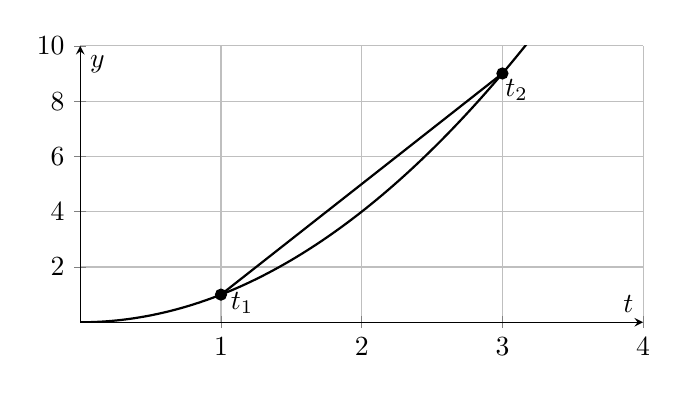
\begin{tikzpicture}
\begin{axis}[
    width=0.72\linewidth,
    height=0.42\linewidth,
    axis lines=middle,
    xlabel={$t$},
    ylabel={$y$},
    xmin=0, xmax=4,
    ymin=0, ymax=10,
    samples=100,
    domain=0:3.2,
    grid=both
]
\addplot[thick] {x^2};
\addplot[thick] coordinates {(1,1) (3,9)};
\addplot[only marks] coordinates {(1,1) (3,9)};
\node at (axis cs:1.15,0.7) {$t_1$};
\node at (axis cs:3.1,8.4) {$t_2$};
\end{axis}
\end{tikzpicture}
\end{center}

\begin{examplebox}{ตัวอย่างที่ 1: อัตราการเปลี่ยนแปลงเฉลี่ย}
กำหนดให้

\[
f(t)=t^2
\]

จงหาอัตราการเปลี่ยนแปลงเฉลี่ยของ $f(t)$ จาก $t=1$ ถึง $t=3$

เริ่มจากนิยาม

\[
\frac{\Delta y}{\Delta t}
=
\frac{f(3)-f(1)}{3-1}
\]

คำนวณค่าฟังก์ชัน

\[
f(3)=9,\quad f(1)=1
\]

แทนค่า

\[
\frac{\Delta y}{\Delta t}
=
\frac{9-1}{2}
\]

\[
\frac{\Delta y}{\Delta t}=4
\]

ดังนั้น

\[
\boxed{4}
\]
\end{examplebox}

% ---------------------------------------------------------
\subsection{ลิมิตและอนุพันธ์}

อัตราการเปลี่ยนแปลงเฉลี่ยใช้จุดสองจุด แต่บางครั้งเราต้องการความชันที่จุดเดียว

ให้จุดแรกอยู่ที่ $t$ และอีกจุดอยู่ที่ $t+\Delta t$

อัตราการเปลี่ยนแปลงเฉลี่ยคือ

\[
\frac{f(t+\Delta t)-f(t)}{\Delta t}
\]

ถ้าทำให้ $\Delta t$ เล็กลงเรื่อย ๆ จนเข้าใกล้ศูนย์ เราได้ความชันที่จุดนั้น

\[
\lim_{\Delta t\to 0}
\frac{f(t+\Delta t)-f(t)}{\Delta t}
\]

ค่าลิมิตนี้เรียกว่า อนุพันธ์ของ $f(t)$

\[
f'(t)=\lim_{\Delta t\to 0}
\frac{f(t+\Delta t)-f(t)}{\Delta t}
\]

\begin{tcolorbox}[title=นิยามของอนุพันธ์]
อนุพันธ์คืออัตราการเปลี่ยนแปลง ณ จุดหนึ่ง หรือความชันของเส้นสัมผัสกราฟที่จุดนั้น
\[
f'(t)=\lim_{\Delta t\to 0}
\frac{f(t+\Delta t)-f(t)}{\Delta t}
\]
\end{tcolorbox}

\begin{center}
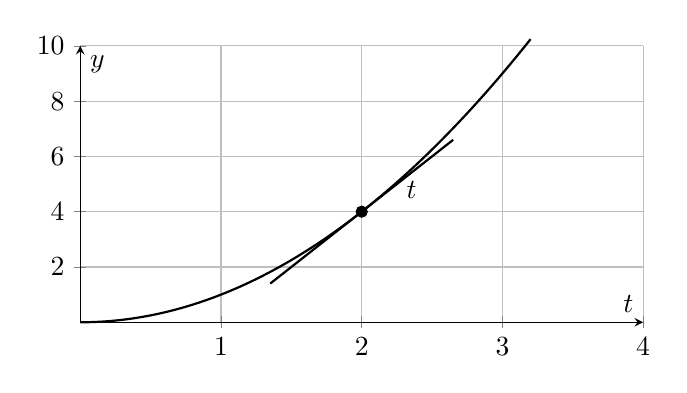
\begin{tikzpicture}
\begin{axis}[
    width=0.72\linewidth,
    height=0.42\linewidth,
    axis lines=middle,
    xlabel={$t$},
    ylabel={$y$},
    xmin=0, xmax=4,
    ymin=0, ymax=10,
    samples=100,
    domain=0:3.2,
    grid=both,
    clip=false
]
\addplot[thick] {x^2};

% Tangent line to y=t^2 at t=2
% Slope = 2t = 4, so tangent is y = 4t - 4
\addplot[thick, domain=1.35:2.65] {4*x - 4};

\addplot[only marks, mark=*] coordinates {(2,4)};

\node[anchor=west] at (axis cs:2.25,4.8) {$t$};
\end{axis}
\end{tikzpicture}
\end{center}

\begin{examplebox}{ตัวอย่างที่ 2: ใช้นิยามอนุพันธ์}
กำหนดให้

\[
f(t)=t^2
\]

จงหา $f'(t)$ จากนิยาม

เริ่มจาก

\[
f'(t)=\lim_{\Delta t\to 0}
\frac{f(t+\Delta t)-f(t)}{\Delta t}
\]

แทนฟังก์ชัน

\[
f'(t)=\lim_{\Delta t\to 0}
\frac{(t+\Delta t)^2-t^2}{\Delta t}
\]

ขยายกำลังสอง

\[
(t+\Delta t)^2=t^2+2t\Delta t+(\Delta t)^2
\]

จึงได้

\[
f'(t)=\lim_{\Delta t\to 0}
\frac{2t\Delta t+(\Delta t)^2}{\Delta t}
\]

ดึง $\Delta t$ เป็นตัวร่วม

\[
f'(t)=\lim_{\Delta t\to 0}
\frac{\Delta t(2t+\Delta t)}{\Delta t}
\]

ตัด $\Delta t$

\[
f'(t)=\lim_{\Delta t\to 0}(2t+\Delta t)
\]

เมื่อ $\Delta t\to 0$

\[
f'(t)=2t
\]

ดังนั้น

\[
\boxed{f'(t)=2t}
\]
\end{examplebox}

% ---------------------------------------------------------
\subsection{กฎอนุพันธ์พื้นฐาน}

\begin{tcolorbox}[title=กฎอนุพันธ์พื้นฐาน]
ถ้า $c$ เป็นค่าคงตัว

\[
\frac{d}{dt}(c)=0
\]

ถ้า $n$ เป็นจำนวนจริง

\[
\frac{d}{dt}(t^n)=nt^{n-1}
\]

ถ้ามีค่าคงตัวคูณอยู่ด้านหน้า

\[
\frac{d}{dt}(ct^n)=cnt^{n-1}
\]

ถ้ามีหลายพจน์ ให้หาอนุพันธ์ทีละพจน์
\end{tcolorbox}

\begin{examplebox}{ตัวอย่างที่ 3: หาอนุพันธ์ทีละพจน์}
กำหนดให้

\[
f(t)=3t^2-2t+5
\]

หาอนุพันธ์อันดับหนึ่ง

\[
f'(t)=\frac{d}{dt}(3t^2-2t+5)
\]

\[
f'(t)=6t-2
\]

หาอนุพันธ์อันดับสอง

\[
f''(t)=\frac{d}{dt}(6t-2)
\]

\[
f''(t)=6
\]

ดังนั้น

\[
\boxed{f'(t)=6t-2}
\]

\[
\boxed{f''(t)=6}
\]
\end{examplebox}

% ---------------------------------------------------------
\subsection{อินทิกรัลและพื้นที่ใต้กราฟ}

ให้กราฟเป็น

\[
y=f(t)
\]

ถ้าแบ่งช่วงจาก $a$ ถึง $b$ ออกเป็นช่วงเล็ก ๆ ที่กว้าง $\Delta t$ พื้นที่เล็กใต้กราฟประมาณได้เป็น

\[
\text{พื้นที่เล็ก}\approx f(t)\Delta t
\]

รวมทุกช่วง

\[
\text{พื้นที่รวม}\approx \sum f(t)\Delta t
\]

เมื่อแบ่งช่วงให้เล็กลงเรื่อย ๆ ผลรวมนี้กลายเป็นอินทิกรัล

\[
\int_a^b f(t)\,dt
\]

\begin{tcolorbox}[title=ความหมายของอินทิกรัล]
\[
\int_a^b f(t)\,dt
\]

คือพื้นที่แบบมีเครื่องหมายใต้กราฟ $y=f(t)$ จาก $t=a$ ถึง $t=b$

ถ้ากราฟอยู่เหนือแกน $t$ พื้นที่จะเป็นบวก

ถ้ากราฟอยู่ใต้แกน $t$ พื้นที่จะเป็นลบ
\end{tcolorbox}

\vspace{1em}
\begin{center}
\begin{tikzpicture}
\begin{axis}[
    width=0.72\linewidth,
    height=0.42\linewidth,
    axis lines=middle,
    xlabel={$t$},
    ylabel={$y$},
    xmin=0, xmax=4,
    ymin=0, ymax=7,
    samples=100,
    domain=0:3.2,
    grid=both
]
\addplot[thick] {2*x+1};
\addplot [
    domain=0.5:3,
    samples=50,
    fill=gray,
    fill opacity=0.25
] {2*x+1} \closedcycle;
\node at (axis cs:1.8,2.0) {พื้นที่};
\end{axis}
\end{tikzpicture}
\end{center}

\subsection{กฎอินทิกรัลพื้นฐาน}

\begin{tcolorbox}[title=กฎอินทิกรัลพื้นฐาน]
ถ้า $n\neq -1$

\[
\int t^n\,dt=\frac{t^{n+1}}{n+1}+C
\]

ถ้า $c$ เป็นค่าคงตัว

\[
\int c\,dt=ct+C
\]

ถ้าเป็นอินทิกรัลจำกัดเขต

\[
\int_a^b f(t)\,dt=F(b)-F(a)
\]

โดยที่

\[
F'(t)=f(t)
\]
\end{tcolorbox}

\begin{examplebox}{ตัวอย่างที่ 4: พื้นที่ใต้กราฟเส้นตรง}
กำหนดให้

\[
f(t)=2t+1
\]

จงหา

\[
\int_0^3 (2t+1)\,dt
\]

หาอินทิกรัลก่อน

\[
\int (2t+1)\,dt=t^2+t+C
\]

ให้

\[
F(t)=t^2+t
\]

ดังนั้น

\[
\int_0^3 (2t+1)\,dt=F(3)-F(0)
\]

\[
F(3)=3^2+3=12
\]

\[
F(0)=0
\]

จึงได้

\[
\boxed{12}
\]
\end{examplebox}

\begin{exercisebox}{แบบฝึกหัดคณิตศาสตร์ก่อนเรียน}
\begin{enumerate}
    \item กำหนดให้ $f(t)=t^2+1$ จงหาอัตราการเปลี่ยนแปลงเฉลี่ยจาก $t=1$ ถึง $t=4$
    \item กำหนดให้ $f(t)=4t^3-2t+7$ จงหา $f'(t)$
    \item กำหนดให้ $f(t)=5t^2-3t+1$ จงหา $f''(t)$
    \item จงหา $\int (6t^2-4)\,dt$
    \item จงหา $\int_0^2 (3t+1)\,dt$
    \item กราฟ $y=f(t)$ เป็นเส้นตรงจากจุด $(0,0)$ ถึง $(4,8)$ จงหาพื้นที่ใต้กราฟจาก $t=0$ ถึง $t=4$
\end{enumerate}
\end{exercisebox}

% =========================================================
\section{ตำแหน่ง ระยะทาง และการกระจัด}

\subsection{ตำแหน่ง}

ก่อนพูดว่าวัตถุเคลื่อนที่อย่างไร เราต้องรู้ก่อนว่าวัตถุอยู่ที่ไหน เมื่อเลือกจุดอ้างอิงและแกนแล้ว เราใช้ $x$ แทนตำแหน่งบนเส้นตรง

ถ้าเลือกจุดกำเนิดเป็น $x=0$ และเลือกทิศขวาเป็นบวก

\[
x=+4\,\si{m}
\]

หมายถึงวัตถุอยู่ทางขวาของจุดกำเนิด $4\,\si{m}$ ส่วน

\[
x=-4\,\si{m}
\]

หมายถึงวัตถุอยู่ทางซ้ายของจุดกำเนิด $4\,\si{m}$

\subsection{การกระจัด}

การกระจัดบอกว่าตำแหน่งเปลี่ยนไปเท่าไรจากต้นทางถึงปลายทาง

\[
\text{การกระจัด}=\text{ตำแหน่งสุดท้าย}-\text{ตำแหน่งเริ่มต้น}
\]

ใช้ $x_i$ แทนตำแหน่งเริ่มต้น และ $x_f$ แทนตำแหน่งสุดท้าย

\[
\Delta x=x_f-x_i
\]

\begin{examplebox}{ตัวอย่าง}
วัตถุเริ่มที่

\[
x_i=-3\,\si{m}
\]

และจบที่

\[
x_f=8\,\si{m}
\]

ดังนั้น

\[
\Delta x=x_f-x_i
\]

\[
\Delta x=8-(-3)=11\,\si{m}
\]

การกระจัดเป็นบวก แปลว่าตำแหน่งสุดท้ายอยู่ทางบวกเมื่อเทียบกับตำแหน่งเริ่มต้น
\end{examplebox}

\subsection{ระยะทาง}

ระยะทางสนใจว่าวัตถุเคลื่อนที่จริงตามเส้นทางทั้งหมดกี่เมตร ไม่สนใจทิศทาง

ถ้าวัตถุไปทางขวา $12\,\si{m}$ แล้วถอยกลับซ้าย $7\,\si{m}$

\[
\text{ระยะทาง}=12+7=19\,\si{m}
\]

แต่การกระจัดคือ

\[
\Delta x=12-7=5\,\si{m}
\]

\begin{tcolorbox}[title=ข้อควรระวัง]
ระยะทางเป็นสเกลาร์ จึงไม่ติดลบ แต่การกระจัดเป็นเวกเตอร์ในแนวตรง จึงเป็นบวก ลบ หรือศูนย์ได้
\end{tcolorbox}

\subsection{ตำแหน่งที่ขึ้นกับเวลา}

บางครั้งตำแหน่งไม่ได้ให้เป็นตัวเลขคงที่ แต่ให้เป็นฟังก์ชันของเวลา เช่น

\[
x(t)=2t^2+3
\]

เมื่อต้องการรู้ตำแหน่งที่เวลาใด ให้แทนค่านั้นลงในฟังก์ชัน

ถ้าเวลาเปลี่ยนจาก $t=1$ เป็น $t=3$ การกระจัดยังคงใช้ความหมายเดิม

\[
\Delta x=x_f-x_i
\]

ในกรณีนี้

\[
x_i=x(1)
\]

และ

\[
x_f=x(3)
\]

คำนวณได้ว่า

\[
x(3)=2(3)^2+3=21
\]

\[
x(1)=2(1)^2+3=5
\]

ดังนั้น

\[
\Delta x=21-5=16\,\si{m}
\]

\begin{tcolorbox}[title=ข้อควรจำ]
แม้ตำแหน่งจะเขียนเป็นฟังก์ชันของเวลา การกระจัดยังคงหมายถึงตำแหน่งสุดท้ายลบตำแหน่งเริ่มต้นเสมอ
\end{tcolorbox}

\begin{exercisebox}{แบบฝึกหัด 2.2}
\begin{enumerate}
    \item อนุภาคเริ่มที่ $x_i=-3\,\si{m}$ และจบที่ $x_f=8\,\si{m}$ จงหาการกระจัด
    \item รถเคลื่อนที่จากตำแหน่ง $x=0$ ไป $x=12\,\si{m}$ แล้วถอยกลับมาที่ $x=5\,\si{m}$ จงหาระยะทางและการกระจัด
    \item วัตถุเคลื่อนที่บนเส้นตรงตามตำแหน่ง $x(t)=t^2-4t+1$ จงหาตำแหน่งเมื่อ $t=0,2,4$
    \item ถ้า $x(t)=3t^2-12t+7$ จงหาช่วงเวลาที่วัตถุกลับมาที่ตำแหน่งเดิมเท่ากับตอน $t=0$
\end{enumerate}
\end{exercisebox}

% =========================================================
\section{อัตราเร็วเฉลี่ย ความเร็วเฉลี่ย และความเร็วขณะหนึ่ง}

\subsection{ความเร็วเฉลี่ย}

เมื่อตำแหน่งของวัตถุเปลี่ยนไป เราต้องการรู้ว่าวัตถุเปลี่ยนตำแหน่งเร็วแค่ไหนในช่วงเวลาหนึ่ง

\[
\text{ความเร็วเฉลี่ย}=\frac{\text{การกระจัด}}{\text{เวลาที่ใช้}}
\]

ดังนั้น

\[
v_{\text{avg}}=\frac{\Delta x}{\Delta t}
\]

เพราะ

\[
\Delta x=x_f-x_i
\]

และ

\[
\Delta t=t_f-t_i
\]

จึงได้

\[
v_{\text{avg}}=\frac{x_f-x_i}{t_f-t_i}
\]

\begin{examplebox}{ตัวอย่าง}
รถเคลื่อนที่จาก

\[
x_i=2\,\si{m}
\]

ไปยัง

\[
x_f=20\,\si{m}
\]

ในเวลา

\[
\Delta t=6\,\si{s}
\]

หาการกระจัดก่อน

\[
\Delta x=20-2=18\,\si{m}
\]

ดังนั้น

\[
v_{\text{avg}}=\frac{18}{6}=3\,\si{m/s}
\]
\end{examplebox}

\subsection{อัตราเร็วเฉลี่ย}

ถ้าไม่สนใจทิศทาง แต่สนใจว่าวัตถุเคลื่อนที่ตามเส้นทางจริงได้เร็วเฉลี่ยเท่าไร ให้ใช้ระยะทางทั้งหมดแทนการกระจัด

\[
\text{อัตราเร็วเฉลี่ย}=\frac{\text{ระยะทางทั้งหมด}}{\text{เวลาทั้งหมด}}
\]

ถ้าให้ระยะทางทั้งหมดเป็น $d$

\[
\text{average speed}=\frac{d}{\Delta t}
\]

\begin{examplebox}{ตัวอย่าง}
นักเรียนเดินไปทางขวา $10\,\si{m}$ ใน $4\,\si{s}$ แล้วเดินกลับซ้าย $6\,\si{m}$ ใน $2\,\si{s}$

ระยะทางรวมคือ

\[
d=10+6=16\,\si{m}
\]

การกระจัดคือ

\[
\Delta x=10-6=4\,\si{m}
\]

เวลารวมคือ

\[
\Delta t=4+2=6\,\si{s}
\]

อัตราเร็วเฉลี่ยคือ

\[
\text{average speed}=\frac{16}{6}=\frac{8}{3}\,\si{m/s}
\]

ความเร็วเฉลี่ยคือ

\[
v_{\text{avg}}=\frac{4}{6}=\frac{2}{3}\,\si{m/s}
\]
\end{examplebox}

\subsection{ความเร็วขณะหนึ่ง}

ความเร็วเฉลี่ยบอกภาพรวมของช่วงเวลา แต่ถ้าต้องการรู้ความเร็ว ณ เวลาหนึ่ง ต้องทำช่วงเวลาให้เล็กลงเรื่อย ๆ

เริ่มจาก

\[
v_{\text{avg}}=\frac{\Delta x}{\Delta t}
\]

เมื่อ

\[
\Delta t\to 0
\]

ค่าเฉลี่ยในช่วงสั้นมากจะกลายเป็นค่าขณะหนึ่ง

\[
v(t)=\lim_{\Delta t\to 0}\frac{\Delta x}{\Delta t}
\]

ในแคลคูลัส เขียนได้ว่า

\[
v(t)=\frac{dx}{dt}
\]

\begin{tcolorbox}[title=การแปลความหมายของเครื่องหมาย]
ถ้า $v(t)>0$ วัตถุเคลื่อนที่ไปทางบวก

ถ้า $v(t)<0$ วัตถุเคลื่อนที่ไปทางลบ

ถ้า $v(t)=0$ วัตถุหยุดชั่วขณะ แต่อาจไม่ได้หยุดถาวร
\end{tcolorbox}

\begin{examplebox}{ตัวอย่าง}
กำหนดให้

\[
x(t)=t^3-6t^2+9t
\]

ต้องการหาเวลาที่วัตถุหยุดชั่วขณะ เงื่อนไขคือ

\[
v(t)=0
\]

แต่ต้องหา $v(t)$ ก่อน

\[
v(t)=\frac{dx}{dt}
\]

ดังนั้น

\[
v(t)=3t^2-12t+9
\]

ให้

\[
3t^2-12t+9=0
\]

หารด้วย $3$

\[
t^2-4t+3=0
\]

แยกตัวประกอบ

\[
(t-1)(t-3)=0
\]

ดังนั้น

\[
t=1\,\si{s},\quad t=3\,\si{s}
\]
\end{examplebox}

\subsection{ความหมายบนกราฟ $x-t$}

ในกราฟตำแหน่งกับเวลา ความเร็วเฉลี่ยคือความชันของเส้นตรงที่ลากระหว่างสองจุด

\[
v_{\text{avg}}=\frac{x(t_2)-x(t_1)}{t_2-t_1}
\]

ถ้ากราฟชันมาก แปลว่าตำแหน่งเปลี่ยนเร็ว

ถ้ากราฟเป็นเส้นราบ แปลว่าตำแหน่งไม่เปลี่ยน

ถ้ากราฟชันขึ้นไปทางขวา ความเร็วเป็นบวก

ถ้ากราฟชันลงไปทางขวา ความเร็วเป็นลบ

\begin{tcolorbox}[title=เชื่อมกับแคลคูลัส]
ถ้าต้องการความเร็ว ณ เวลาใดเวลาหนึ่ง ให้ดูความชันของเส้นสัมผัสกราฟที่เวลานั้น ซึ่งเขียนได้เป็น

\[
v(t)=\frac{dx}{dt}
\]
\end{tcolorbox}

\begin{exercisebox}{แบบฝึกหัด 2.3}
\begin{enumerate}
    \item รถเคลื่อนที่จาก $x=2\,\si{m}$ ไป $x=20\,\si{m}$ ในเวลา $6\,\si{s}$ จงหาความเร็วเฉลี่ย
    \item เด็กเดินทางไปทางขวา $4\,\si{m}$ แล้วเดินกลับซ้าย $4\,\si{m}$ ในเวลา $5\,\si{s}$ จงหาความเร็วเฉลี่ยและอัตราเร็วเฉลี่ย
    \item ถ้า $x(t)=5t^2+2t-1$ จงหา $v(t)$ และ $v(3)$
    \item ถ้า $x(t)=t^3-3t^2-9t$ จงหาเวลาที่วัตถุหยุดชั่วขณะ
    \item วัตถุมีตำแหน่ง $x(t)=2t^3-15t^2+36t$ จงพิจารณาว่าวัตถุเคลื่อนที่ไปทางบวกหรือลบในช่วง $0<t<5$
\end{enumerate}
\end{exercisebox}

% =========================================================
\section{ความเร่ง}

\subsection{ความเร่งเฉลี่ย}

หลังจากรู้ว่าความเร็วคืออัตราการเปลี่ยนตำแหน่ง คำถามต่อมาคือ ความเร็วเปลี่ยนเร็วแค่ไหน ปริมาณนี้เรียกว่า ความเร่ง

\[
\text{ความเร่งเฉลี่ย}=\frac{\text{การเปลี่ยนความเร็ว}}{\text{เวลาที่ใช้}}
\]

การเปลี่ยนความเร็วคือ

\[
\Delta v=v_f-v_i
\]

ดังนั้น

\[
a_{\text{avg}}=\frac{\Delta v}{\Delta t}
\]

หรือ

\[
a_{\text{avg}}=\frac{v_f-v_i}{t_f-t_i}
\]

\subsection{ความเร่งขณะหนึ่ง}

ความเร่งขณะหนึ่งได้จากการทำช่วงเวลาให้สั้นลงจนเข้าใกล้ศูนย์

\[
a(t)=\lim_{\Delta t\to 0}\frac{\Delta v}{\Delta t}
\]

ในแคลคูลัสคือ

\[
a(t)=\frac{dv}{dt}
\]

และเพราะ

\[
v(t)=\frac{dx}{dt}
\]

ดังนั้น

\[
a(t)=\frac{d^2x}{dt^2}
\]

\begin{tcolorbox}[title=กฎจำง่าย]
ถ้า $v$ และ $a$ มีเครื่องหมายเดียวกัน วัตถุเร็วขึ้น

ถ้า $v$ และ $a$ มีเครื่องหมายตรงข้าม วัตถุช้าลง

ถ้า $a=0$ ความเร็วคงตัว

ถ้า $v=0$ ไม่ได้แปลว่า $a=0$
\end{tcolorbox}

\begin{examplebox}{ตัวอย่าง}
วัตถุมีตำแหน่ง

\[
x(t)=2t^3-5t^2+4t
\]

หาความเร็ว

\[
v(t)=\frac{dx}{dt}
\]

\[
v(t)=6t^2-10t+4
\]

หาความเร่ง

\[
a(t)=\frac{dv}{dt}
\]

\[
a(t)=12t-10
\]
\end{examplebox}

\subsection{ความหมายบนกราฟ $v-t$}

ในกราฟความเร็วกับเวลา ความเร่งคือความชันของกราฟ

\[
a_{\text{avg}}=\frac{\Delta v}{\Delta t}
\]

ถ้ากราฟ $v-t$ ชันขึ้น ความเร่งเป็นบวก

ถ้ากราฟ $v-t$ ชันลง ความเร่งเป็นลบ

ถ้ากราฟ $v-t$ เป็นเส้นราบ ความเร่งเป็นศูนย์ และความเร็วคงตัว

\begin{tcolorbox}[title=เชื่อมกับแคลคูลัส]
ถ้าต้องการความเร่ง ณ เวลาใดเวลาหนึ่ง ให้ดูความชันของเส้นสัมผัสกราฟ $v-t$ ที่เวลานั้น ซึ่งเขียนได้เป็น

\[
a(t)=\frac{dv}{dt}
\]
\end{tcolorbox}

\begin{exercisebox}{แบบฝึกหัด 2.4}
\begin{enumerate}
    \item รถเพิ่มความเร็วจาก $5\,\si{m/s}$ เป็น $25\,\si{m/s}$ ในเวลา $4\,\si{s}$ จงหาความเร่งเฉลี่ย
    \item วัตถุมี $v(t)=4t^2-3t+2$ จงหา $a(t)$
    \item วัตถุมี $x(t)=t^4-4t^2+3$ จงหา $v(t)$ และ $a(t)$
    \item ถ้า $v=-6\,\si{m/s}$ และ $a=2\,\si{m/s^2}$ วัตถุกำลังเร็วขึ้นหรือช้าลง
    \item ถ้า $a(t)=2t+3$ และ $v(0)=1$ จงหา $v(t)$
\end{enumerate}
\end{exercisebox}

% =========================================================
\section{การเคลื่อนที่ด้วยความเร่งคงตัว}

\subsection{เงื่อนไขสำคัญ}

สมการในส่วนนี้ใช้ได้เมื่อความเร่งคงตัวเท่านั้น

\[
a=\text{constant}
\]

ถ้าความเร่งไม่คงตัว ต้องใช้แคลคูลัสหรือวิธีอื่น ไม่ควรนำสูตรชุดนี้ไปใช้ทันที

\subsection{สมการที่ 1: ความเร็วปลาย}

เริ่มจากนิยามของความเร่งเฉลี่ย

\[
a=\frac{\Delta v}{\Delta t}
\]

เมื่อความเร่งคงตัว และให้เริ่มจับเวลาที่ $t=0$

\[
a=\frac{v_f-v_i}{t}
\]

จัดรูป

\[
v_f-v_i=at
\]

ดังนั้น

\[
v_f=v_i+at
\]

\begin{tcolorbox}[title=สมการที่ 1]
\[
v_f=v_i+at
\]

ใช้เมื่อรู้ความเร็วต้น ความเร่ง และเวลา
\end{tcolorbox}

\subsection{สมการที่ 2: การกระจัดจากพื้นที่ใต้กราฟ $v-t$}

เมื่อความเร่งคงตัว กราฟ $v-t$ เป็นเส้นตรง เพราะความเร็วเปลี่ยนอย่างสม่ำเสมอ

การกระจัดเท่ากับพื้นที่ใต้กราฟ $v-t$

\[
\Delta x=\text{area under }v-t
\]

พื้นที่ใต้กราฟเส้นตรงเป็นรูปสี่เหลี่ยมคางหมู

\[
\Delta x=\frac{1}{2}(v_i+v_f)t
\]

ดังนั้น

\[
x_f-x_i=\frac{v_i+v_f}{2}t
\]

\begin{tcolorbox}[title=สมการที่ 2]
\[
\Delta x=\frac{v_i+v_f}{2}t
\]

ใช้เมื่อรู้ความเร็วต้น ความเร็วปลาย และเวลา
\end{tcolorbox}

\subsection{สมการที่ 3: การกระจัดเมื่อไม่รู้ความเร็วปลาย}

เริ่มจากสมการที่ 2

\[
\Delta x=\frac{v_i+v_f}{2}t
\]

ใช้สมการที่ 1

\[
v_f=v_i+at
\]

แทนค่า $v_f$ ลงไป

\[
\Delta x=\frac{v_i+(v_i+at)}{2}t
\]

รวมพจน์

\[
\Delta x=\frac{2v_i+at}{2}t
\]

กระจาย $t$

\[
\Delta x=v_it+\frac{1}{2}at^2
\]

ดังนั้น

\[
x_f=x_i+v_it+\frac{1}{2}at^2
\]

\begin{tcolorbox}[title=สมการที่ 3]
\[
\Delta x=v_it+\frac{1}{2}at^2
\]

ใช้เมื่อรู้ความเร็วต้น ความเร่ง และเวลา แต่ไม่ต้องใช้ความเร็วปลาย
\end{tcolorbox}

\subsection{สมการที่ 4: ความเร็วกับการกระจัดเมื่อไม่รู้เวลา}

เริ่มจากสมการที่ 1

\[
v_f=v_i+at
\]

จัดรูปเพื่อหาเวลา

\[
t=\frac{v_f-v_i}{a}
\]

นำไปแทนในสมการที่ 2

\[
\Delta x=\frac{v_i+v_f}{2}t
\]

จะได้

\[
\Delta x=\frac{v_i+v_f}{2}\left(\frac{v_f-v_i}{a}\right)
\]

ใช้ผลต่างกำลังสอง

\[
(v_i+v_f)(v_f-v_i)=v_f^2-v_i^2
\]

ดังนั้น

\[
\Delta x=\frac{v_f^2-v_i^2}{2a}
\]

จัดรูป

\[
v_f^2-v_i^2=2a\Delta x
\]

จึงได้

\[
v_f^2=v_i^2+2a\Delta x
\]

\begin{tcolorbox}[title=สมการที่ 4]
\[
v_f^2=v_i^2+2a\Delta x
\]

ใช้เมื่อโจทย์ไม่ต้องการเวลา หรือไม่ได้ให้เวลา
\end{tcolorbox}

\subsection{วิธีเลือกสูตร}

\begin{enumerate}
    \item กำหนดแกนและทิศบวก
    \item เขียนสิ่งที่รู้ เช่น $v_i$, $v_f$, $a$, $t$, $\Delta x$
    \item เขียนสิ่งที่ต้องหา
    \item เลือกสมการที่มีสิ่งที่ต้องหา และไม่มีตัวแปรที่โจทย์ไม่ให้
\end{enumerate}

\begin{examplebox}{ตัวอย่าง}
รถเริ่มจากหยุดนิ่งและเร่งด้วยความเร่งคงตัว $2\,\si{m/s^2}$ เป็นเวลา $5\,\si{s}$ จงหาระยะทาง

แปลโจทย์

\[
v_i=0,\quad a=2\,\si{m/s^2},\quad t=5\,\si{s}
\]

ต้องการหา

\[
\Delta x
\]

ไม่ต้องรู้ $v_f$ จึงใช้

\[
\Delta x=v_it+\frac{1}{2}at^2
\]

แทนค่า

\[
\Delta x=(0)(5)+\frac{1}{2}(2)(5^2)
\]

\[
\Delta x=25\,\si{m}
\]
\end{examplebox}

\subsection{อ่านเสริม: ที่มาของสมการจากแคลคูลัส}

\begin{tcolorbox}[title=หมายเหตุสำหรับผู้เรียน]
ส่วนนี้ใช้แคลคูลัสเพื่อพิสูจน์ว่าสมการการเคลื่อนที่มาจากนิยามจริง ๆ ถ้ายังไม่คล่องแคลคูลัส สามารถข้ามก่อน แล้วกลับมาอ่านหลังจากทำโจทย์พื้นฐานได้
\end{tcolorbox}

เริ่มจากนิยามของความเร่งขณะหนึ่ง

\[
a=\frac{dv}{dt}
\]

จัดรูป

\[
dv=a\,dt
\]

ถ้า $a$ คงตัว อินทิเกรตจาก $v_i$ ถึง $v_f$ และจาก $0$ ถึง $t$

\[
\int_{v_i}^{v_f}dv=\int_0^t a\,dt
\]

\[
v_f-v_i=at
\]

ดังนั้น

\[
v_f=v_i+at
\]

ต่อไปเริ่มจากนิยามของความเร็ว

\[
v=\frac{dx}{dt}
\]

จัดรูป

\[
dx=v\,dt
\]

เพราะ

\[
v=v_i+at
\]

แทนลงไป

\[
dx=(v_i+at)\,dt
\]

อินทิเกรต

\[
\int_{x_i}^{x_f}dx=\int_0^t (v_i+at)\,dt
\]

\[
x_f-x_i=v_it+\frac{1}{2}at^2
\]

ดังนั้น

\[
\Delta x=v_it+\frac{1}{2}at^2
\]

\begin{exercisebox}{แบบฝึกหัด 2.5}
\begin{enumerate}
    \item รถเริ่มจากหยุดนิ่ง เร่งด้วย $3\,\si{m/s^2}$ เป็นเวลา $4\,\si{s}$ จงหาความเร็วสุดท้ายและระยะทาง
    \item วัตถุมี $v_i=10\,\si{m/s}$ และชะลอด้วย $a=-2\,\si{m/s^2}$ จงหาเวลาที่หยุด
    \item รถเคลื่อนที่ด้วย $v_i=5\,\si{m/s}$ และมี $a=2\,\si{m/s^2}$ จนความเร็วเป็น $15\,\si{m/s}$ จงหาระยะทาง
    \item วัตถุเคลื่อนที่จากหยุดนิ่งด้วยความเร่งคงตัว ระยะทางในวินาทีที่ 4 เท่ากับเท่าไร ถ้า $a=2\,\si{m/s^2}$
    \item รถ A เริ่มจากหยุดนิ่งด้วยความเร่ง $2a$ รถ B เริ่มพร้อมกันจากหยุดนิ่งด้วยความเร่ง $a$ จงหาอัตราส่วนระยะทางของ A ต่อ B หลังเวลาผ่านไปเท่ากัน
\end{enumerate}
\end{exercisebox}

% =========================================================
\section{การตกอิสระ}

\subsection{แนวคิดหลัก}

การตกอิสระคือการเคลื่อนที่ที่มีแรงโน้มถ่วงเป็นสาเหตุหลักของความเร่ง โดยละเลยแรงต้านอากาศ ใกล้ผิวโลกใช้ค่าประมาณ

\[
g\approx 9.8\,\si{m/s^2}
\]

ทิศของความเร่งโน้มถ่วงชี้ลงเสมอ

ถ้าเลือกแกนขึ้นเป็นบวก

\[
a=-g
\]

ถ้าเลือกแกนลงเป็นบวก

\[
a=+g
\]

\begin{tcolorbox}[title=จุดสำคัญ]
ที่จุดสูงสุดของการโยนขึ้นในแนวดิ่ง ความเร็วเป็นศูนย์ชั่วขณะ แต่ความเร่งยังชี้ลง ดังนั้นถ้าเลือกขึ้นเป็นบวก ความเร่งยังเป็น $-g$
\end{tcolorbox}

\subsection{สมการตกอิสระจากสมการความเร่งคงตัว}

การตกอิสระใกล้ผิวโลกเป็นกรณีพิเศษของการเคลื่อนที่ด้วยความเร่งคงตัว

ถ้าเลือกแกนขึ้นเป็นบวก จะมี

\[
a=-g
\]

จากสมการเดิม

\[
v_f=v_i+at
\]

แทน $a=-g$

\[
v_f=v_i-gt
\]

จาก

\[
\Delta y=v_it+\frac{1}{2}at^2
\]

แทน $a=-g$

\[
\Delta y=v_it-\frac{1}{2}gt^2
\]

หรือ

\[
y_f=y_i+v_it-\frac{1}{2}gt^2
\]

\begin{examplebox}{ตัวอย่าง}
โยนวัตถุขึ้นด้วยความเร็วต้น $20\,\si{m/s}$ จงหาความสูงสูงสุด ใช้ $g=10\,\si{m/s^2}$

เลือกแกนขึ้นเป็นบวก

\[
v_i=20\,\si{m/s}
\]

ที่จุดสูงสุด

\[
v_f=0
\]

ความเร่งคือ

\[
a=-10\,\si{m/s^2}
\]

ต้องการหาความสูง จึงใช้สมการที่ไม่มีเวลา

\[
v_f^2=v_i^2+2a\Delta y
\]

แทนค่า

\[
0^2=20^2+2(-10)\Delta y
\]

\[
0=400-20\Delta y
\]

\[
20\Delta y=400
\]

\[
\Delta y=20\,\si{m}
\]
\end{examplebox}

\begin{tcolorbox}[title=ข้อควรจำ]
โจทย์ตกอิสระส่วนใหญ่ไม่ยากเพราะสูตร แต่ยากเพราะเลือกเครื่องหมายผิด ให้กำหนดแกนก่อนทุกครั้ง
\end{tcolorbox}

\begin{exercisebox}{แบบฝึกหัด 2.6}
\begin{enumerate}
    \item ปล่อยวัตถุจากหยุดนิ่งจากความสูง $45\,\si{m}$ ใช้ $g=10\,\si{m/s^2}$ จงหาเวลาตกถึงพื้น
    \item โยนวัตถุขึ้นด้วย $30\,\si{m/s}$ ใช้ $g=10\,\si{m/s^2}$ จงหาความสูงสูงสุด
    \item จากข้อก่อนหน้า จงหาเวลารวมที่วัตถุกลับมาระดับเดิม
    \item ปล่อยหินจากตึกสูง $80\,\si{m}$ และหลังจากนั้น $1\,\si{s}$ โยนหินอีกก้อนลงด้วยความเร็วต้น $10\,\si{m/s}$ จงหาว่าก้อนใดถึงพื้นก่อน
    \item วัตถุถูกโยนขึ้นจากพื้น เมื่อเวลาผ่านไป $2\,\si{s}$ และ $4\,\si{s}$ วัตถุอยู่ที่ความสูงเท่ากัน ใช้ $g=10\,\si{m/s^2}$ จงหาความเร็วต้นและความสูงนั้น
\end{enumerate}
\end{exercisebox}

% =========================================================
\section{กราฟการเคลื่อนที่}

\subsection{กราฟตำแหน่งกับเวลา}

เริ่มจากนิยามของความเร็วเฉลี่ย

\[
v_{\text{avg}}=\frac{\Delta x}{\Delta t}
\]

ในกราฟ $x-t$ ค่า

\[
\frac{\Delta x}{\Delta t}
\]

คือความชันของกราฟ ดังนั้นความชันของกราฟ $x-t$ คือความเร็ว

\begin{tcolorbox}[title=สรุปกราฟ $x-t$]
ความชันของกราฟ $x-t$ คือความเร็ว
\end{tcolorbox}

\subsection{กราฟความเร็วกับเวลา}

เริ่มจากนิยามของความเร่งเฉลี่ย

\[
a_{\text{avg}}=\frac{\Delta v}{\Delta t}
\]

ในกราฟ $v-t$ ค่า

\[
\frac{\Delta v}{\Delta t}
\]

คือความชันของกราฟ ดังนั้นความชันของกราฟ $v-t$ คือความเร่ง

ต่อไป จากแนวคิดพื้นที่ใต้กราฟ ถ้าความเร็วคงที่ในช่วงเวลาสั้น ๆ

\[
\Delta x\approx v\Delta t
\]

เมื่อนำทุกช่วงมารวมกัน จะได้ว่าพื้นที่ใต้กราฟ $v-t$ คือการกระจัด

\[
\Delta x=\text{area under }v-t
\]

\begin{tcolorbox}[title=สรุปกราฟ $v-t$]
ความชันของกราฟ $v-t$ คือความเร่ง

พื้นที่ใต้กราฟ $v-t$ คือการกระจัด
\end{tcolorbox}

\subsection{กราฟความเร่งกับเวลา}

จากความหมายของความเร่ง

\[
a\approx \frac{\Delta v}{\Delta t}
\]

จัดรูป

\[
\Delta v\approx a\Delta t
\]

เมื่อนำทุกช่วงมารวมกัน จะได้ว่าพื้นที่ใต้กราฟ $a-t$ คือการเปลี่ยนความเร็ว

\[
\Delta v=\text{area under }a-t
\]

\begin{tcolorbox}[title=สรุปกราฟ $a-t$]
พื้นที่ใต้กราฟ $a-t$ คือการเปลี่ยนความเร็ว
\end{tcolorbox}

\subsection{สรุปการอ่านกราฟ}

\[
\text{ความชันของกราฟ }x-t=\text{ความเร็ว}
\]

\[
\text{ความชันของกราฟ }v-t=\text{ความเร่ง}
\]

\[
\text{พื้นที่ใต้กราฟ }v-t=\text{การกระจัด}
\]

\[
\text{พื้นที่ใต้กราฟ }a-t=\text{การเปลี่ยนความเร็ว}
\]

\begin{tcolorbox}[title=ข้อควรจำ]
กราฟเป็นเครื่องมือสำคัญมากในข้อสอบ เพราะบางครั้งโจทย์ไม่ได้ให้สมการ แต่ให้รูปกราฟแทน นักเรียนต้องอ่านความชันและพื้นที่ให้เป็น
\end{tcolorbox}

\begin{exercisebox}{แบบฝึกหัด 2.7}
\begin{enumerate}
    \item กราฟ $v-t$ เป็นเส้นตรงจาก $v=0$ ถึง $v=20\,\si{m/s}$ ใน $5\,\si{s}$ จงหาการกระจัด
    \item กราฟ $a-t$ มี $a=4\,\si{m/s^2}$ คงตัวเป็นเวลา $3\,\si{s}$ ถ้า $v_i=2\,\si{m/s}$ จงหา $v_f$
    \item ถ้า $v(t)=6t-4$ จงหาการกระจัดจาก $t=1$ ถึง $t=3$
    \item ถ้า $a(t)=2t$ และ $v(0)=3$ จงหา $v(4)$
    \item ถ้า $x(t)=t^3-6t^2+12t$ จงวิเคราะห์ช่วงที่วัตถุเร็วขึ้นและช้าลงในช่วง $0<t<5$
\end{enumerate}
\end{exercisebox}

% =========================================================
\section{ชุดโจทย์รวมท้ายบท: คละระดับสำหรับ สอวน. ค่าย 1}

\subsection*{ระดับพื้นฐาน}

\begin{enumerate}
    \item วัตถุเคลื่อนที่จาก $x=-5\,\si{m}$ ไป $x=15\,\si{m}$ ใน $4\,\si{s}$ จงหาความเร็วเฉลี่ย
    \item วัตถุเริ่มจากหยุดนิ่งด้วยความเร่ง $2\,\si{m/s^2}$ เป็นเวลา $10\,\si{s}$ จงหาระยะทาง
    \item โยนวัตถุขึ้นด้วย $20\,\si{m/s}$ ใช้ $g=10\,\si{m/s^2}$ จงหาเวลาถึงจุดสูงสุด
    \item วัตถุมี $x(t)=4t^2-3t+1$ จงหา $v(t)$ และ $a(t)$
\end{enumerate}

\subsection*{ระดับกลาง}

\begin{enumerate}
    \setcounter{enumi}{4}
    \item รถเริ่มจากหยุดนิ่งและวิ่งด้วยความเร่งคงตัว ระยะทางในวินาทีที่ 5 เท่ากับ $18\,\si{m}$ จงหาความเร่ง
    \item วัตถุมี $v(t)=t^2-4t+3$ จงหาการกระจัดจาก $t=0$ ถึง $t=5$
    \item โยนวัตถุขึ้นจากพื้นด้วยความเร็วต้น $u$ จงพิสูจน์ว่าความสูงสูงสุดคือ
    \[
    H=\frac{u^2}{2g}
    \]
    \item รถสองคันเริ่มจากจุดเดียวกัน รถ A เริ่มจากหยุดนิ่งด้วยความเร่ง $a$ รถ B ออกตัวด้วยความเร็วคงตัว $u$ จงหาเวลาที่ A ตามทัน B
\end{enumerate}

\subsection*{ระดับยาก}

\begin{enumerate}
    \setcounter{enumi}{8}
    \item วัตถุเคลื่อนที่ตาม
    \[
    x(t)=t^3-9t^2+24t
    \]
    จงหาเวลาที่วัตถุเปลี่ยนทิศทาง และหาตำแหน่งที่เกิดเหตุการณ์นั้น

    \item วัตถุเริ่มที่ $x=0$ และ $v=0$ โดยมีความเร่ง
    \[
    a(t)=6t-4
    \]
    จงหา $x(t)$

    \item ลิฟต์กำลังเคลื่อนที่ขึ้นด้วยความเร็ว $v_0$ เมื่อวัตถุหลุดจากมือคนในลิฟต์ จงเขียนสมการตำแหน่งของวัตถุเทียบกับพื้นโลก โดยเลือกแกนขึ้นเป็นบวก

    \item ลูกบอลถูกโยนขึ้นจากพื้นด้วยความเร็วต้น $u$ หลังจากเวลาผ่านไป $T$ ลูกบอลอยู่ที่ความสูง $h$ จงหาค่า $u$ ในรูปของ $h,T,g$

    \item รถคันหนึ่งเคลื่อนที่ด้วยความเร็วต้น $u$ แล้วเบรกด้วยความเร่งขนาด $a$ จนหยุด ระยะหยุดคือ $s$ ถ้าความเร็วต้นเพิ่มเป็น $2u$ และความเร่งเบรกมีขนาดเท่าเดิม ระยะหยุดเป็นกี่เท่าของเดิม

    \item วัตถุเคลื่อนที่โดยมี
    \[
    v(x)=kx
    \]
    เมื่อ $k$ เป็นค่าคงตัวบวก จงหา $x(t)$ ถ้า $x(0)=x_0$
\end{enumerate}

% =========================================================
\section{เฉลยย่อท้ายบท}

\begin{enumerate}
    \item
    \[
    v_{\text{avg}}=\frac{15-(-5)}{4}=5\,\si{m/s}
    \]

    \item
    \[
    \Delta x=\frac{1}{2}at^2=\frac{1}{2}(2)(10^2)=100\,\si{m}
    \]

    \item
    ที่จุดสูงสุด $v_f=0$
    \[
    0=20-10t
    \]
    \[
    t=2\,\si{s}
    \]

    \item
    \[
    v(t)=8t-3
    \]
    \[
    a=8\,\si{m/s^2}
    \]

    \item
    ระยะทางในวินาทีที่ $n$ จากหยุดนิ่งคือ
    \[
    s_n=\frac{1}{2}a(2n-1)
    \]
    เมื่อ $n=5$
    \[
    18=\frac{1}{2}a(9)
    \]
    \[
    a=4\,\si{m/s^2}
    \]

    \item
    \[
    \Delta x=\int_0^5 (t^2-4t+3)\,dt
    \]
    \[
    \Delta x=\left[\frac{t^3}{3}-2t^2+3t\right]_0^5
    \]
    \[
    \Delta x=\frac{125}{3}-50+15
    \]
    \[
    \Delta x=\frac{20}{3}\,\si{m}
    \]

    \item
    ที่จุดสูงสุด
    \[
    v_f=0
    \]
    ใช้
    \[
    v_f^2=v_i^2+2a\Delta y
    \]
    โดย $a=-g$ และ $\Delta y=H$
    \[
    0=u^2-2gH
    \]
    \[
    H=\frac{u^2}{2g}
    \]

    \item
    \[
    x_A=\frac{1}{2}at^2
    \]
    \[
    x_B=ut
    \]
    ตามทันเมื่อ
    \[
    \frac{1}{2}at^2=ut
    \]
    ไม่คิดคำตอบ $t=0$
    \[
    t=\frac{2u}{a}
    \]

    \item
    \[
    v(t)=\frac{dx}{dt}=3t^2-18t+24
    \]
    \[
    v(t)=3(t-2)(t-4)
    \]
    เปลี่ยนทิศที่
    \[
    t=2,\quad t=4
    \]
    ตำแหน่งคือ
    \[
    x(2)=8-36+48=20
    \]
    \[
    x(4)=64-144+96=16
    \]

    \item
    \[
    v(t)=\int(6t-4)\,dt=3t^2-4t+C
    \]
    ใช้ $v(0)=0$ ได้ $C=0$
    \[
    v(t)=3t^2-4t
    \]
    ต่อไป
    \[
    x(t)=\int(3t^2-4t)\,dt=t^3-2t^2+C_2
    \]
    ใช้ $x(0)=0$ ได้ $C_2=0$
    \[
    x(t)=t^3-2t^2
    \]

    \item
    เลือกแกนขึ้นเป็นบวก
    \[
    y(t)=y_0+v_0t-\frac{1}{2}gt^2
    \]
    โดย $v_0$ คือความเร็วของลิฟต์ขณะปล่อย

    \item
    \[
    h=uT-\frac{1}{2}gT^2
    \]
    ดังนั้น
    \[
    u=\frac{h}{T}+\frac{1}{2}gT
    \]

    \item
    ระยะหยุด
    \[
    s=\frac{u^2}{2a}
    \]
    ถ้าความเร็วต้นเป็น $2u$
    \[
    s'=\frac{(2u)^2}{2a}=4s
    \]
    ดังนั้นระยะหยุดเป็น $4$ เท่า

    \item
    จาก
    \[
    v=\frac{dx}{dt}=kx
    \]
    แยกตัวแปร
    \[
    \frac{dx}{x}=k\,dt
    \]
    อินทิเกรต
    \[
    \ln x=kt+C
    \]
    ใช้ $x(0)=x_0$
    \[
    x(t)=x_0e^{kt}
    \]
\end{enumerate}

% =========================================================
\section{สรุปสูตรสำคัญ}

\begin{tcolorbox}[title=สรุปบท: การเคลื่อนที่แนวตรง]
\[
\Delta x=x_f-x_i
\]

\[
v_{\text{avg}}=\frac{\Delta x}{\Delta t}
\]

\[
\text{average speed}=\frac{\text{total distance}}{\Delta t}
\]

\[
v=\frac{dx}{dt}
\]

\[
a_{\text{avg}}=\frac{\Delta v}{\Delta t}
\]

\[
a=\frac{dv}{dt}=\frac{d^2x}{dt^2}
\]

เมื่อ $a$ คงตัว

\[
v_f=v_i+at
\]

\[
\Delta x=\frac{v_i+v_f}{2}t
\]

\[
\Delta x=v_it+\frac{1}{2}at^2
\]

\[
v_f^2=v_i^2+2a\Delta x
\]

ตกอิสระใกล้ผิวโลก ถ้าเลือกแกนขึ้นเป็นบวก

\[
a=-g
\]

\[
v_f=v_i-gt
\]

\[
\Delta y=v_it-\frac{1}{2}gt^2
\]
\end{tcolorbox}

% =========================================================
\section{ข้อสอบจริง สอวน. ที่ใช้ความรู้บทการเคลื่อนที่แนวตรง}


% =========================================================
\subsection{ปี 2560 ข้อ 2: กระดานลื่นที่ความชันค่อย ๆ ลดลง}
\vspace{1.5em}
\IfFileExists{img/posn60q2.png}{
\begin{center}
    \includegraphics[width=1\linewidth]{img/posn60q2.png}
\end{center}
}

\begin{examplebox}{เฉลยแนวคิด}
โจทย์พูดถึงกระดานลื่นที่ช่วงบนชันมาก แล้วค่อย ๆ ลดความชันลงที่ปลายล่าง ต้องพิจารณาสองอย่าง

\[
\text{ขนาดของความเร็ว}
\]

และ

\[
\text{ขนาดของความเร่ง}
\]

ถ้าวัตถุยังเคลื่อนที่ลงตามกระดานและยังถูกเร่งไปข้างหน้า ความเร็วจะยังเพิ่มขึ้น

\[
v \text{ เพิ่มขึ้น}
\]

แต่เมื่อกระดานค่อย ๆ ลดความชันลง องค์ประกอบของความเร่งตามแนวกระดานจะลดลง เพราะกระดานเข้าใกล้แนวราบมากขึ้น

\[
a \text{ ลดลง}
\]

สรุปคือ

\[
\boxed{\text{ขนาดของความเร็วเพิ่มขึ้น แต่ขนาดของความเร่งลดลง}}
\]

\[
\boxed{\text{ตอบ D}}
\]
\end{examplebox}

% =========================================================
\subsection{ปี 2560 ข้อ 3: หลอดไฟตกในลิฟต์ที่เร่งขึ้น}
\vspace{1.5em}
\IfFileExists{img/posn60q3.png}{
\begin{center}
    \includegraphics[width=1\linewidth]{img/posn60q3.png}
\end{center}
}

\vspace{1.5em}
\begin{examplebox}{เฉลยละเอียด}
ลิฟต์เคลื่อนที่ขึ้นด้วยความเร่งคงตัว

\[
a_{\text{lift}}=+2.0\,\si{m/s^2}
\]

หลอดไฟอยู่สูงจากพื้นลิฟต์

\[
h=2.95\,\si{m}
\]

เมื่อหลอดไฟหลุดจากเพดาน หลอดไฟและพื้นลิฟต์มีความเร็วต้นเท่ากันในขณะนั้น เพราะก่อนหลุดทั้งสองเคลื่อนที่ไปพร้อมกับลิฟต์

ดังนั้นความเร็วสัมพัทธ์เริ่มต้นระหว่างหลอดไฟกับพื้นลิฟต์คือ

\[
v_{\text{rel},0}=0
\]

เลือกแกนขึ้นเป็นบวก

หลอดไฟมีความเร่ง

\[
a_{\text{bulb}}=-g
\]

พื้นลิฟต์มีความเร่ง

\[
a_{\text{floor}}=+2.0
\]

ดังนั้นความเร่งของหลอดไฟเทียบกับพื้นลิฟต์คือ

\[
a_{\text{rel}}=a_{\text{bulb}}-a_{\text{floor}}
\]

\[
a_{\text{rel}}=-g-2.0
\]

ใช้ $g=9.8\,\si{m/s^2}$

\[
a_{\text{rel}}=-11.8\,\si{m/s^2}
\]

พิจารณาขนาดของการปิดระยะห่าง

\[
h=\frac{1}{2}(g+2.0)t^2
\]

แทนค่า

\[
2.95=\frac{1}{2}(11.8)t^2
\]

\[
2.95=5.9t^2
\]

\[
t^2=\frac{2.95}{5.9}
\]

\[
t^2=\frac{1}{2}
\]

ดังนั้น

\[
\boxed{t=\frac{1}{\sqrt{2}}\,\si{s}}
\]
\end{examplebox}


% =========================================================
\subsection{ปี 2561 ข้อ 3: ลูกเทนนิสสามลูกถูกโยนขึ้นในแนวดิ่ง}
\vspace{1.5em}
\IfFileExists{img/posn61q3.png}{
\begin{center}
    \includegraphics[width=1\linewidth]{img/posn61q3.png}
\end{center}
}

\vspace{1em}
\begin{examplebox}{เฉลยละเอียด}
ลูกเทนนิสแต่ละลูกถูกโยนขึ้นจากตำแหน่งเดียวกัน ด้วยความเร็วต้นเท่ากัน

\[
u=9.80\,\si{m/s}
\]

และเว้นช่วงเวลาระหว่างลูกถัดไป

\[
1.00\,\si{s}
\]

ต้องการหาความสูงที่ลูกที่ 2 และลูกที่ 3 สวนกัน

ให้เริ่มนับเวลา $t$ จากขณะที่โยนลูกที่ 2

ตำแหน่งของลูกที่ 2 คือ

\[
y_2=ut-\frac{1}{2}gt^2
\]

ลูกที่ 3 ถูกโยนหลังลูกที่ 2 เป็นเวลา $1\,\si{s}$ ดังนั้นเวลาที่ลูกที่ 3 เคลื่อนที่คือ

\[
t-1
\]

ตำแหน่งของลูกที่ 3 คือ

\[
y_3=u(t-1)-\frac{1}{2}g(t-1)^2
\]

เมื่อสวนกัน

\[
y_2=y_3
\]

แทนสมการ

\[
ut-\frac{1}{2}gt^2
=
u(t-1)-\frac{1}{2}g(t-1)^2
\]

จัดรูป

\[
u=\frac{1}{2}g\left[t^2-(t-1)^2\right]
\]

เพราะ

\[
t^2-(t-1)^2=2t-1
\]

จึงได้

\[
u=\frac{1}{2}g(2t-1)
\]

แทน $u=g=9.80$

\[
g=\frac{1}{2}g(2t-1)
\]

ตัด $g$

\[
1=\frac{1}{2}(2t-1)
\]

\[
2=2t-1
\]

\[
t=\frac{3}{2}\,\si{s}
\]

หาความสูงจากสมการของลูกที่ 2

\[
y_2=ut-\frac{1}{2}gt^2
\]

\[
y_2=9.8\left(\frac{3}{2}\right)-\frac{1}{2}(9.8)\left(\frac{3}{2}\right)^2
\]

\[
y_2=14.7-11.025
\]

\[
y_2=3.675\,\si{m}
\]

ดังนั้นประมาณเป็น

\[
\boxed{3.7\,\si{m}}
\]
\end{examplebox}

% =========================================================
\subsection{ปี 2561 ตอนที่ 2 ข้อ 1: บั้งไฟเร่งขึ้นแล้วเชื้อเพลิงหมด}

\vspace{1.5em}
\IfFileExists{img/posn61s2q1.png}{
\begin{center}
    \includegraphics[width=1\linewidth]{img/posn61s2q1.png}
\end{center}
}

\vspace{1.5em}

\begin{examplebox}{เฉลยละเอียด}
บั้งไฟเริ่มจากหยุดนิ่ง และเร่งขึ้นด้วยความเร่ง

\[
a=+g
\]

เป็นเวลา

\[
t=10\,\si{s}
\]

แบ่งการเคลื่อนที่เป็นสองช่วง

\[
\text{ช่วงที่ 1: เชื้อเพลิงยังทำงาน}
\]

\[
\text{ช่วงที่ 2: เชื้อเพลิงหมดและเคลื่อนที่ต่อภายใต้แรงโน้มถ่วง}
\]

\textbf{ช่วงที่ 1}

เริ่มจากหยุดนิ่ง

\[
v_i=0
\]

ระยะที่ขึ้นในช่วงแรกคือ

\[
s_1=v_it+\frac{1}{2}at^2
\]

\[
s_1=0+\frac{1}{2}g(10)^2
\]

\[
s_1=50g
\]

ความเร็วเมื่อเชื้อเพลิงหมดคือ

\[
v_1=v_i+at
\]

\[
v_1=10g
\]

\textbf{ช่วงที่ 2}

หลังเชื้อเพลิงหมด บั้งไฟยังเคลื่อนที่ขึ้นต่อ แต่มีความเร่งลง

\[
a=-g
\]

ที่จุดสูงสุด

\[
v_f=0
\]

ใช้

\[
v_f^2=v_i^2+2a\Delta y
\]

โดยช่วงที่ 2 มี

\[
v_i=10g
\]

ดังนั้น

\[
0=(10g)^2+2(-g)s_2
\]

\[
2gs_2=100g^2
\]

\[
s_2=50g
\]

ความสูงสูงสุดจากพื้นคือ

\[
H=s_1+s_2
\]

\[
H=50g+50g=100g
\]

ถ้าใช้

\[
g=9.8\,\si{m/s^2}
\]

จะได้

\[
\boxed{H=980\,\si{m}}
\]
\end{examplebox}

% =========================================================
\subsection{ปี 2567 ข้อ 10: เรือเข้าใกล้หน้าผาและเสียงสะท้อน}
\vspace{1.5em}
\IfFileExists{img/posn67q10.png}{
\begin{center}
    \includegraphics[width=1\linewidth]{img/posn67q10.png}
\end{center}
}
\vspace{1.5em}
\begin{examplebox}{เฉลยละเอียด}
ให้เรือเคลื่อนที่เข้าหาหน้าผาด้วยความเร็วคงตัว

\[
v
\]

และเสียงมีอัตราเร็วในอากาศ

\[
c
\]

คนบนเรือได้ยินเสียงสะท้อนหลังจากเปิดหวูดเป็นเวลา

\[
t
\]

ให้ระยะเริ่มต้นจากเรือถึงหน้าผาเป็น

\[
D
\]

ในเวลา $t$ เสียงเดินทางได้ระยะ

\[
ct
\]

ในเวลาเดียวกัน เรือเคลื่อนที่เข้าใกล้หน้าผาได้ระยะ

\[
vt
\]

ดังนั้นตอนเสียงสะท้อนกลับมาถึงเรือ ระยะจากเรือถึงหน้าผาจะเหลือ

\[
D-vt
\]

เสียงเดินทางสองช่วง

\[
\text{ไปหน้าผา}=D
\]

\[
\text{กลับมาถึงเรือ}=D-vt
\]

ระยะรวมของเสียงคือ

\[
ct=D+(D-vt)
\]

\[
ct=2D-vt
\]

จัดรูป

\[
(c+v)t=2D
\]

ดังนั้น

\[
D=\frac{(c+v)t}{2}
\]

เวลาที่เรือจะชนหน้าผาหลังจากเปิดหวูดคือ

\[
T=\frac{D}{v}
\]

แทนค่า $D$

\[
T=\frac{1}{v}\left(\frac{(c+v)t}{2}\right)
\]

ดังนั้น

\[
\boxed{T=\frac{(c+v)t}{2v}}
\]
\end{examplebox}

% =========================================================
\subsection{ปี 2568 ข้อ 18: เรือแล่นหนีจากหน้าผาและเสียงสะท้อน}

\vspace{1.5em}
\IfFileExists{img/posn68q18.png}{
\begin{center}
    \includegraphics[width=1\linewidth]{img/posn68q18.png}
\end{center}
}{
\begin{tcolorbox}[title=ตำแหน่งภาพที่แนะนำ]
ให้ตัดภาพข้อสอบปี 2568 ข้อ 18 แล้วบันทึกเป็น

\[
\texttt{img/posn68q18.png}
\]
\end{tcolorbox}
}

\vspace{1.5em}

\begin{examplebox}{เฉลยละเอียด}
โจทย์นี้เป็นการเคลื่อนที่แนวตรงแบบความเร็วคงตัว โดยมีเสียงเดินทางไปกลับระหว่างเรือกับหน้าผา

ให้เรือแล่นหนีจากหน้าผาด้วยความเร็วคงตัว

\[
v
\]

อัตราเร็วเสียงในอากาศคือ

\[
c
\]

เรือเริ่มแล่นหนีจากหน้าผาเมื่อเวลา

\[
t=0
\]

และเปิดหวูดเมื่อเวลา

\[
t=t_1
\]

ดังนั้นขณะเปิดหวูด ระยะระหว่างเรือกับหน้าผาคือ

\[
d=vt_1
\]

หลังจากเปิดหวูด คนบนเรือได้ยินเสียงสะท้อนเมื่อเวลาผ่านไป

\[
\tau
\]

ในช่วงเวลา $\tau$ เสียงเดินทางได้ระยะทั้งหมด

\[
c\tau
\]

แต่เรือยังแล่นหนีหน้าผาต่อไปอีก ดังนั้นในช่วงเวลา $\tau$ เรือเคลื่อนที่เพิ่มอีก

\[
v\tau
\]

พิจารณาระยะทางที่เสียงเดินทาง

\[
\text{ช่วงที่ 1: จากเรือไปหน้าผา}=d
\]

\[
\text{ช่วงที่ 2: จากหน้าผากลับไปหาเรือ}=d+v\tau
\]

ดังนั้นระยะรวมของเสียงคือ

\[
c\tau=d+(d+v\tau)
\]

แทน

\[
d=vt_1
\]

จะได้

\[
c\tau=vt_1+(vt_1+v\tau)
\]

\[
c\tau=2vt_1+v\tau
\]

ดึง $v$ เป็นตัวร่วม

\[
c\tau=v(2t_1+\tau)
\]

ดังนั้นความเร็วของเรือคือ

\[
\boxed{v=\frac{c\tau}{2t_1+\tau}}
\]
\end{examplebox}


% =========================================================
\subsection{ปี 2565 ข้อ 28: เรือเข้าใกล้หน้าผาและเสียงสะท้อนสองครั้ง}

\vspace{1.5em}

\IfFileExists{img/posn65q28.png}{
\begin{center}
    \includegraphics[width=1\linewidth]{img/posn65q28.png}
\end{center}
}{
\begin{tcolorbox}[title=ตำแหน่งภาพที่แนะนำ]
ให้ตัดภาพข้อสอบปี 2565 ข้อ 28 แล้วบันทึกเป็น

\[
\texttt{img/posn65q28.png}
\]

ข้อนี้เหมาะกับบทการเคลื่อนที่สองมิติในหัวข้อความเร็วสัมพัทธ์ หรือใช้เป็นข้อเสริมท้ายบทการเคลื่อนที่แนวตรง เพราะแกนหลักคือการตั้งสมการระยะทางของเสียงและระยะทางของเรือ
\end{tcolorbox}
}

\vspace{1.5em}

\begin{examplebox}{เฉลยละเอียด}
ให้เรือเคลื่อนที่เข้าหาหน้าผาด้วยความเร็วคงตัว

\[
v
\]

และให้อัตราเร็วเสียงในอากาศเป็น

\[
c
\]

ที่ตำแหน่ง 1 เรือเปิดหวูด แล้วคนบนเรือได้ยินเสียงสะท้อนหลังเวลา

\[
t_1
\]

หลังจากเรือเคลื่อนที่จากตำแหน่ง 1 ไปยังตำแหน่ง 2 เป็นเวลา

\[
\tau
\]

เรือเปิดหวูดอีกครั้ง แล้วคนบนเรือได้ยินเสียงสะท้อนหลังเวลา

\[
t_2
\]

ให้ระยะจากตำแหน่ง 1 ถึงหน้าผาเป็น

\[
D_1
\]

และระยะจากตำแหน่ง 2 ถึงหน้าผาเป็น

\[
D_2
\]

เพราะเรือเคลื่อนที่เข้าหาหน้าผาด้วยความเร็ว $v$ เป็นเวลา $\tau$

\[
D_2=D_1-v\tau
\]

\textbf{ครั้งที่ 1}

เสียงเดินทางจากเรือไปถึงหน้าผา แล้วสะท้อนกลับมาหาเรือ

ในเวลา $t_1$ เสียงเดินทางได้ระยะ

\[
ct_1
\]

ในเวลาเดียวกัน เรือเคลื่อนที่เข้าหาหน้าผาได้ระยะ

\[
vt_1
\]

ดังนั้นระยะทางรวมที่เสียงเดินทางคือ

\[
D_1+(D_1-vt_1)
\]

จึงได้

\[
ct_1=2D_1-vt_1
\]

จัดรูป

\[
(c+v)t_1=2D_1
\]

ดังนั้น

\[
D_1=\frac{(c+v)t_1}{2}
\]

\textbf{ครั้งที่ 2}

ที่ตำแหน่ง 2 ระยะเริ่มต้นถึงหน้าผาคือ $D_2$

ในทำนองเดียวกัน

\[
ct_2=2D_2-vt_2
\]

จัดรูป

\[
(c+v)t_2=2D_2
\]

ดังนั้น

\[
D_2=\frac{(c+v)t_2}{2}
\]

แต่จากความสัมพันธ์ของระยะ

\[
D_2=D_1-v\tau
\]

แทนค่า $D_1$ และ $D_2$

\[
\frac{(c+v)t_2}{2}
=
\frac{(c+v)t_1}{2}
-
v\tau
\]

คูณทั้งสมการด้วย $2$

\[
(c+v)t_2=(c+v)t_1-2v\tau
\]

ย้ายข้าง

\[
(c+v)(t_1-t_2)=2v\tau
\]

กระจายซ้ายมือ

\[
c(t_1-t_2)+v(t_1-t_2)=2v\tau
\]

ย้ายพจน์ที่มี $v$ ไปรวมกัน

\[
c(t_1-t_2)=2v\tau-v(t_1-t_2)
\]

ดึง $v$ เป็นตัวร่วม

\[
c(t_1-t_2)=v\left[2\tau-(t_1-t_2)\right]
\]

ดังนั้น

\[
v=
\frac{c(t_1-t_2)}
{2\tau-(t_1-t_2)}
\]

หรือเขียนอีกแบบได้เป็น

\[
\boxed{
v=
\frac{c(t_1-t_2)}
{2\tau+t_2-t_1}
}
\]

\begin{tcolorbox}[title=ตรวจความสมเหตุสมผล]
เพราะเรือเข้าใกล้หน้าผา ระยะทางครั้งที่ 2 สั้นกว่าครั้งที่ 1 ดังนั้นเวลารอเสียงสะท้อนควรลดลง

\[
t_1>t_2
\]

และตัวส่วนต้องเป็นบวก

\[
2\tau+t_2-t_1>0
\]

คำตอบจึงมีความหมายทางฟิสิกส์
\end{tcolorbox}
\end{examplebox}
